\vspace{-2em}
\section{Περιγραφή προβλήματος}
\label{Problem Description}
Σκοπός της συγκεκριμένης εργασίας ήταν η χρήση δύο διαφορετικών συνόλων δεδομένων (dataset) και η εκπαίδευση νευρωνικών δικτύων για κάθε ένα από αυτά. Επιπλέον το πρώτο μοντέλο θα έπρεπε να χρησιμοποιηθεί ως βάση για την εφαρμογή της μεθόδου της μεταφοράς μάθησης (transfer learning) κατά την εκπαίδευση του δεύτερου δικτύου. Η επιλογή των συνόλων δεδομένων και του τύπου του προβλήματος (π.χ. παλινδρόμηση, ταξινόμηση κλπ.) που χρησιμοποιήθηκαν ήταν ελεύθερη. 

Για τη συγκεκριμένη εργασία, επιλέχθηκε ένα πρόβλημα ταξινόμησης πολλών κλάσεων (multiclass classification), όπου με τη χρήση εικόνων γίνεται διάκριση μεταξύ διαφορετικών ειδών τροφής. Τα δύο datasets που χρησιμοποιήθηκαν είναι το UECFOOD256 \cite{kaggle_dataset_UECFOOD256} και το FOOD101 \cite{kaggle_dataset_FOOD101}.

Πιο συγκεκριμένα, το πρώτο dataset περιλαμβάνει περίπου 31000 φωτογραφίες 256 διαφορετικών τροφών με διαφορετικό αριθμό φωτογραφιών για κάθε μια από τις 256 κατηγορίες, με τις περισσότερες εξ αυτών να είναι κατηγορίες τροφών που συναντώνται στην Ιαπωνία. Στο δεύτερο σύνολο δεδομένων εντοπίζονται 101 κλάσεις με 1000 ακριβώς φωτογραφίες ανά κλάση. 

Τα δύο σύνολα έχουν κάποια κοινά στοιχεία, πχ υπάρχει η κλάση "πίτσα" και στα δύο, αλλά η μεγάλη πλειοψηφία των κλάσεων ανήκει αποκλειστικά σε ένα από τα δύο σύνολα. Η λογική που ακολουθήθηκε ήταν να επιλεγεί το πρώτο dataset και να εκπαιδευτεί πάνω σε αυτό ένας ταξινομητής (classifier) με όσο το δυνατόν μεγαλύτερη ακρίβεια πρόβλεψης του είδους της τροφής και εν συνεχεία να χρησιμοποιηθεί για μεταφορά μάθησης στο δεύτερο dataset. Στον πίνακα \ref{Food_datasets_table} παρατίθενται τα στοιχεία για το μέγεθος και τον αριθμό των κλάσεων των συνόλων δεδομένων που χρησιμοποιήθηκαν.

\begin{table}[H]
\centering
\begin{tabular}{|c|c|c|}
\hline
                & UECFOOD256 & FOOD101 \\ \hline
Κλάσεις         & 256        & 101     \\ \hline
Αριθμός εικόνων & 31651      & 101000  \\ \hline
\end{tabular}
\caption{Σύνολα δεδομένων (datasets)}
\label{Food_datasets_table}
\end{table}


\section{Περιγραφή παραδοτέου προγράμματος}
\label{Package Structure}

Πριν την αναλυτική περιγραφή των βημάτων που ακολουθήθηκαν για την εκπαίδευση των νευρωνικών δικτύων παρατίθεται μια σύντομη περιγραφή της δομής του παραδοτέου πακέτου κώδικα ώστε να υπάρχει μια εικόνα της σύνδεσης όλων όσων περιγράφονται στο υπόλοιπο κείμενο. Στο σχήμα \ref{Package_Structure_image} φαίνεται η δομή του παραδοτέου προγράμματος. Τα βασικά στοιχεία συνοψίζονται στα εξής.

\begin{enumerate}
\item dummy\_data: Φάκελος που περιέχει δεδομένα ΧΧΧΧΧΧΧ
\item logs :  Φάκελος ο οποίος δημιουργείται κατά τη διάρκεια της πρώτης εκτέλεσης του προγράμματος και περιέχει log αρχεία με χρήσιμες πληροφορίες για την πορεία εκτέλεσης του προγράμματος
\item myenv : Φάκελος που περιέχει το εικονικό περιβάλλον το οποίο χρησιμοποιήθηκε για την ανάπτυξη του κώδικα. Η ενεργοποίηση του γίνεται με βάση τις οδηγίες που υπάρχουν στο README αρχείο 
\item py\_imports :  Φάκελος που περιέχει τα διάφορα python scripts (κλάσεις, συναρτήσεις) που χρησιμοποιούνται στο κυρίως πρόγραμμα
\item py\_plots :  Φάκελος που περιέχει τις συναρτήσεις (κώδικας python) που χρησιμοποιούνται για τη δημιουργία διαφόρων σχημάτων και γραφικών παραστάσεων που χρησιμοποιούνται στην παρούσα αναφορά
\item results : Φάκελος αποτελεσμάτων που δημιουργείται κατά την πρώτη εκτέλεση του προγράμματος
\item main.py : Κυρίως πρόγραμμα python
\item .gitignore, README, environment : Αρχεία του git και του εικονικού περιβάλλοντος
\end{enumerate}


\begin{figure}[H]
\centering
\begin{subfigure}[t]{0.3\textwidth}%
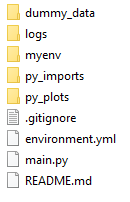
\includegraphics[width=\textwidth]{Program_Structure.png}
\end{subfigure}
\caption{Δομή προγράμματος}
\label{Package_Structure_image}
\end{figure}


\section{Προεπεξεργασία δεδομένων}
\label{Data pre-processing}

Οι εικόνες και των δύο dataset είναι διαφόρων διαστάσεων και αναλογιών πλάτους-ύψους, οπότε πριν την εκκίνηση της εκπαίδευσης παρεμβάλλεται υποχρεωτικά ένα βήμα προ-επεξεργασίας κατά το οποίο όλες οι εικόνες αποκτούν τις ίδιες διαστάσεις. Για τον σκοπό αυτό αναπτύχθηκε κώδικας ο οποίος αναλαμβάνει την μετατροπή των εικόνων στο επιθυμητό τελικό μέγεθος.

Επιπλέον, στο σύνολο δεδομένων UECFOOD256 δίνονται τα περιγράμματα (bounding boxes) που περικλείουν το είδος της τροφής προς ταξινόμηση και αποκλείουν όλο το περιβάλλον. Γίνεται λοιπόν χρήση μιας μεθόδου αποκοπής (cropping), ώστε να μείνει μόνο το συγκεκριμένο αντικείμενο εντός εικόνας και να διευκολυνθεί η διαδικασία της εκπαίδευσης επιτυγχάνοντας τελικά μεγαλύτερη ακρίβεια πρόβλεψης. Στην εικόνα \ref{Crop_image} φαίνεται το αποτέλεσμα της αποκοπής σε μια εικόνα του UECFOOD256. Σε όλες τις περιπτώσεις επιλέχθηκε η διατήρηση και των τριών καναλιών χρωμάτων σε κάθε εικόνα και η μη μετατροπή τους σε μονοχρωματικές για λόγους επίτευξης μεγαλύτερης ακρίβειας κατά τη διάρκεια της εκπαίδευσης, παρά το αυξημένο υπολογιστικό κόστος που αυτή η απόφαση συνεπάγεται.

\begin{figure}[H]
\centering
\begin{subfigure}[t]{0.5\textwidth}%
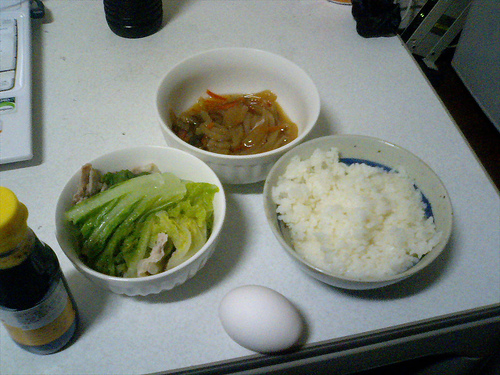
\includegraphics[width=\textwidth]{εικόνα_πριν.jpg}
\caption{Πριν}
\end{subfigure}%
\begin{subfigure}[t]{0.5\textwidth}%
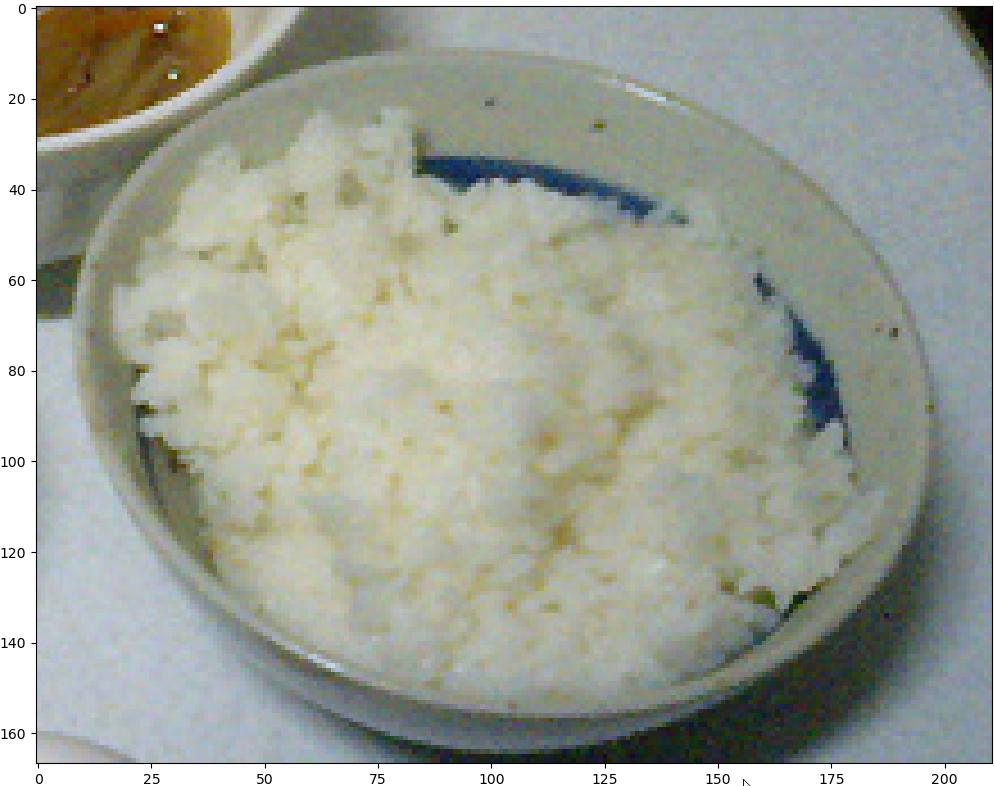
\includegraphics[width=\textwidth]{εικόνα_μετά.png}
\caption{Μετά}
\end{subfigure} 
\caption{UECFOOD256 αποκοπή εικόνας}
\label{Crop_image}
\end{figure}

Επιπλέον η ύπαρξη των bounding boxes ήταν και ο βασικός λόγος που επιλέχθηκε το συγκεκριμένο σύνολο δεδομένων ως αρχικό και όχι το FOOD101, όπως ήταν η αρχική πρόθεση, καθώς προτιμήθηκε η λογική της εκπαίδευσης του μοντέλου σε ένα "καθαρό" σύνολο δεδομένων το οποίο περιέχει περισσότερες κλάσεις αλλά παράλληλα λιγότερες εικόνες ανά κλάση, ώστε να εκτεθεί το μοντέλο σε πολλά διαφορετικά είδη τροφών και να αναπτύξει με αυτό τον τρόπο τη δυνατότητα να εντοπίζει συγκεκριμένα χαρακτηριστικά στοιχεία (features), τα οποία και θα μπορούσαν να χρησιμοποιηθούν σε ένα άλλο σύνολο δεδομένων για την ταξινόμηση τροφών. 

Αντίθετα στο δεύτερο σύνολο δεδομένων δεν είναι διαθέσιμα αυτά τα πλαίσια εντοπισμού και για αυτό τον λόγο δεν είναι δυνατή η απομόνωση και αποκοπή της εικόνας του φαγητού, ενώ αναφέρεται ότι έχει γίνει και λανθασμένη απόδοση κλάσης σε μερικές από τις εικόνες, πράγμα που επηρεάζει αρνητικά το τελικό αποτέλεσμα.

Ένα ακόμη στοιχείο που αξίζει σχολιασμού είναι ότι η προ-επεξεργασία των εικόνων είναι μια αρκετά χρονοβόρα διαδικασία η οποία ξεπερνάει τη μια ώρα για κάθε σύνολο δεδομένων, οπότε επελέγη οι εικόνες να επεξεργαστούν μια φορά για κάθε επιλεγόμενη διάσταση πχ (128, 128) και να αποθηκευτούν σε αρχεία τύπου .h5. Στη συνέχεια κάθε φορά που το πρόγραμμα εκτελείτο οι εικόνες διαβάζονταν απευθείας από τα αρχεία και εισάγονταν στο πρόγραμμα ως πίνακες (numpy.arrays) τύπου int8.

Τέλος μετά την προ-επεξεργασία και αποθήκευση των εικόνων γίνεται ο διαχωρισμός των δεδομένων σε training-validation-test set με αναλογίες 70\%-15\%-15\% και είναι πλέον δυνατή η εκτέλεση του επόμενου βήματος που αφορά την εκπαίδευση του νευρωνικού δικτύου. 